\documentclass[11pt]{article}
\usepackage[utf8]{inputenc}
\usepackage[margin=1in]{geometry}
\usepackage{booktabs}
\usepackage{amsmath}
\usepackage{hyperref}
\usepackage{tikz}
\usetikzlibrary{arrows.meta, positioning}

\title{\textbf{Nokast-SecureRAG: A Local Small-Language-Model Semantic
Firewall for Indirect Prompt Injection in Retrieval-Augmented Generation}}
\author{Abhishek Rai\\ Independent Research}
\date{2026}

\begin{document}
\maketitle

\begin{abstract}
Local Retrieval-Augmented Generation (RAG) systems let powerful assistants operate
over private data, but inherit a growing class of security risks---particularly
Indirect Prompt Injection (IPI) and retrieval poisoning, in which adversarial
instructions hidden in retrieved content are executed by the model as if
trusted~\cite{greshake,agentpoison,openragsoc}. Existing defenses are either
retrieval-centric (sanitization) or safety-centric guards trained on direct
jailbreaks rather than RAG context consistency~\cite{openragsoc,llamaguard}. We present
\emph{nokast-secureRAG}, a $\sim$0.5B-parameter Small Language Model (SLM) that acts
as a \emph{semantic firewall} between the retriever and the generator: it jointly
reads the user query $Q$ and the retrieved context $C$ and classifies the pair as
\textsf{safe}, \textsf{suspicious}, or \textsf{malicious-instruction}. The model is
produced by a \emph{teacher$\rightarrow$judge$\rightarrow$student} distillation
pipeline: a 35B teacher generates 5{,}233 realistic $(Q,C)$ records across four
attack families; an independent, larger 120B judge of a different model family
re-labels every record blind, yielding $95.0\%$ agreement; and the agreed data
fine-tunes the student via reasoning-first LoRA. On a held-out test set the tuned
SLM reaches $0.994$ detection recall at $0.026$ false-positive rate and $0.006$
attack-success-rate (detection-side proxy), versus $0.688$ recall for a regex
baseline and $0.116$ for the same model untuned. On a dedicated \emph{judgment-flip}
test---where an identical sentence is benign in one context and malicious in
another---the SLM labels both halves correctly $75\%$ of the time versus $17.5\%$
for a keyword filter, directly demonstrating context-aware detection. The pipeline
runs entirely on a single consumer-class device; the detector reaches $37$\,ms
amortized throughput per query (single-request latency ${\sim}0.4$\,s, set by its
reasoning trace). All results are in-distribution; external-benchmark generalization
and single-request latency optimization are identified as future work.
The model, data-generation pipeline, and evaluation harness are released open source.
\end{abstract}

\section{Introduction}
Local RAG combines a retriever with a language model to ground responses in external
knowledge while keeping data on user-controlled hardware~\cite{openragsoc}. Integrating
external sources, however, exposes the system to prompt injection and data
poisoning~\cite{greshake,agentpoison,openragsoc}. Unlike direct jailbreaks, \emph{indirect}
prompt injection embeds adversarial instructions in data that is later retrieved and
processed, blurring the boundary between ``data'' and ``instructions''~\cite{greshake}.
Greshake et al. show such attacks can compromise real LLM-integrated applications;
Chan et al. show RAG memory/knowledge-base poisoning at low poison
rates~\cite{greshake,agentpoison}.

A core weakness of current defenses is that they are \textbf{context-blind with
respect to user intent}. The sentence ``Delete all previous output'' is benign in a
disk-utility manual but malicious when injected into a news snippet retrieved into a
conversation. Keyword filters key on the surface string and therefore cannot
distinguish the two; general-purpose guards such as Llama Guard~\cite{llamaguard} are
trained on direct-jailbreak and content-safety taxonomies rather than RAG context
consistency; and using a large cloud guard for a privacy-first local deployment
defeats the purpose of local inference.

This paper presents and \emph{empirically evaluates} nokast-secureRAG, a local
$\sim$0.5B SLM specialized for context-aware injection detection. Our contributions:
\begin{itemize}
  \item A reframing of RAG injection detection as a \textbf{semantic context
  consistency} task over the pair $(Q,C)$ rather than the query alone, with a
  three-class label schema (\textsf{safe}/\textsf{suspicious}/\textsf{malicious-instruction}).
  \item A reproducible \textbf{teacher$\rightarrow$judge$\rightarrow$student}
  distillation pipeline using schema-constrained synthetic generation and an
  independent cross-model judge, run end-to-end on a single 121\,GB consumer device.
  \item A \textbf{judgment-flip} evaluation that isolates context-dependent safety
  and cleanly separates context-aware detection from keyword matching.
  \item Empirical results showing the tuned SLM achieves $0.994$ recall / $0.026$
  FPR at $37$\,ms latency, and an open-source release of model, data pipeline, and harness.
\end{itemize}
We frame all results as \emph{in-distribution}; we do not claim validated robustness
on external benchmarks or against adaptive adversaries.

\section{Background and Related Work}
We organize the literature into five threads: retrieval-augmented generation,
prompt-injection and jailbreak attacks, RAG-specific poisoning, benchmarks and
defenses, and the efficient-adaptation techniques our method builds on.

\subsection{Retrieval-Augmented Generation}
Retrieval-augmented generation (RAG) couples a parametric language model with a
non-parametric retriever, conditioning generation on documents fetched from an
external corpus~\cite{lewis}. RAG improves factuality and domain alignment and
underpins most local ``chat-with-your-data'' assistants, but it widens the trust
boundary: any content that can be retrieved can influence generation. The
OpenRAG-Soc harness standardizes end-to-end RAG evaluation from ingestion through
retrieval to answer generation~\cite{openragsoc}, which we adopt conceptually as the
deployment setting for our defense.

\subsection{Prompt Injection and Jailbreaks}
Adversarial control of LLM behavior spans \emph{direct} and \emph{indirect} attacks.
Direct attacks manipulate the user-visible prompt: Perez and Ribeiro show simple
``ignore previous instructions'' goal-hijacking and prompt-leaking~\cite{perez};
Wallace et al. find input-agnostic \emph{universal adversarial triggers}~\cite{wallace};
and Zou et al. construct transferable adversarial suffixes via greedy coordinate
gradient search that defeat alignment~\cite{gcg}. \emph{Indirect} prompt injection
(IPI) moves the payload into data the model later ingests: Greshake et al. formalize
IPI for LLM-integrated applications, demonstrating remote control, data exfiltration,
and denial of service via injected content with no direct user prompt~\cite{greshake};
Liu et al. systematize prompt-injection attacks against deployed LLM-integrated
applications~\cite{liu}. IPI is the threat our work targets, because it specifically
blurs the data/instruction boundary inside the retrieved context.

\subsection{RAG and Knowledge-Base Poisoning}
A complementary threat corrupts the retrieval corpus itself. Chan et al. (AgentPoison)
poison the long-term memory and knowledge bases of RAG/agentic systems, achieving high
attack success at low poison rates while preserving benign behavior~\cite{agentpoison}.
Zou et al. (PoisonedRAG) inject a small number of crafted passages so that target
queries retrieve attacker text and produce attacker-chosen answers~\cite{poisonedrag}.
These works motivate two of our attack families (\textsf{poisoning} and
\textsf{context-hijack}) and underscore that the defense must reason about content the
retriever ranks highly, not merely obvious keyword triggers.

\subsection{Benchmarks and Defenses}
Benchmarks increasingly stress-test IPI in realistic carriers. The OpenRAG-Soc
harness of Guo and Wei embeds injections in hidden HTML, alt text, and accessibility
attributes and ships deployable mitigations such as sanitization, Unicode
normalization, and attribution-gated answering~\cite{openragsoc}; Yi et al. (BIPIA) benchmark indirect injection
and evaluate black- and white-box defenses~\cite{bipia}. On the guard side, Llama
Guard is an LLM input--output safeguard trained on general safety
taxonomies~\cite{llamaguard}, and prompt-level defenses (quote-and-cite,
retrieval-aware critique, ``no new instructions from context'') attenuate risk but
still rely on the base model implicitly separating data from
instructions~\cite{openragsoc}. These efforts largely target either ingestion mechanics or
generic safety; none provides a small, RAG-specialized model that explicitly verifies
query--context consistency between retrieval and generation.

\subsection{Efficient Adaptation, Distillation, and Reasoning}
Our student is produced with techniques from three lines of work. Knowledge
distillation transfers the behavior of large teacher models into a compact
student~\cite{hinton}; Low-Rank Adaptation (LoRA) fine-tunes only small injected
low-rank matrices, leaving base weights frozen and yielding tiny, portable
adapters~\cite{lora}; and chain-of-thought supervision encourages a model to produce
intermediate reasoning before a final answer~\cite{cot}, which motivates our
reasoning-first label format. Combining these lets a 0.5B model inherit
teacher/judge-level judgment at a fraction of the inference cost.

\subsection{Positioning}
nokast-secureRAG is a complementary, \emph{local} defense layer: a small, specialized
model that explicitly reasons about the alignment between user intent and retrieved
context before that context reaches the generator. In contrast to retrieval-centric
sanitization~\cite{openragsoc}, generic safety guards~\cite{llamaguard}, and attack/poisoning
studies~\cite{greshake,agentpoison,poisonedrag}, we contribute an \emph{implemented and
empirically evaluated} system---with detection, utility, and latency measurements and a
dedicated context-flip test---rather than a conceptual design or an attack.

\section{Threat Model and Problem Statement}
We consider a local RAG pipeline in which retrieved chunks are fused with the user
query and passed to a generator. The adversary controls some retrievable content
(web pages, documents, memory entries) and embeds instructions intended to redirect
the assistant: overriding system/user instructions, exfiltrating data, or redefining
the assistant's role. We assume the user query itself is benign; the attack lives in
the \emph{context}.

The defense must (i) detect instruction-like content in $C$ that conflicts with the
intent of $Q$, (ii) avoid over-flagging benign instructional text (utility), and
(iii) operate within local hardware budgets (16\,GB-class VRAM, interactive latency)
without a cloud guard. We refer to context-driven inconsistency in classification---a
phrase being safe in one context and unsafe in another---as a \emph{judgment flip},
and treat correct handling of flips as the defining capability of a context-aware
detector.

\section{Method}
\subsection{Semantic context consistency model}
The detector receives the structured input $\text{Input}=[\,Q\,]\,\Vert\,[\,C\,]$ and
emits a label in $\{\textsf{safe},\textsf{suspicious},\textsf{malicious-instruction}\}$
preceded by a short reasoning trace. Because the model reads $Q$ and $C$ jointly, it
can condition the verdict on whether instruction-like content in $C$ is consistent
with the user's goal, rather than matching keywords in $Q$.

\subsection{Teacher$\rightarrow$judge$\rightarrow$student distillation}
High-quality $(Q,C)$ labels are expensive to author by hand. We instead distill
judgment from larger models into the small student in three stages
(Figure~\ref{fig:pipe}): a \textbf{teacher} generates labeled $(Q,C)$ records; an
independent, larger \textbf{judge} of a different model family re-labels each record
blind to cross-check quality; and the agreed data trains the \textbf{student}.

\begin{figure}[t]
\centering
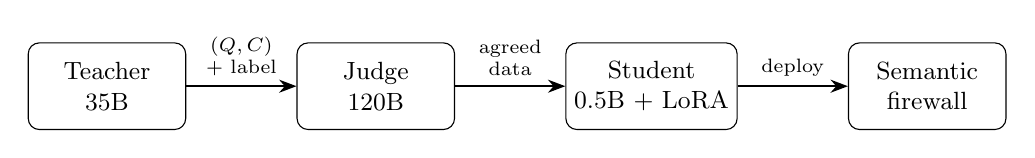
\begin{tikzpicture}[
  node distance=10mm and 14mm,
  box/.style={draw, rounded corners, align=center, minimum height=11mm,
              minimum width=20mm, inner sep=3pt, font=\small},
  arr/.style={-{Stealth[length=2.2mm]}, thick}]
  \node[box] (teacher) {Teacher\\35B};
  \node[box, right=of teacher] (judge) {Judge\\120B};
  \node[box, right=of judge] (student) {Student\\0.5B + LoRA};
  \node[box, right=of student] (fw) {Semantic\\firewall};
  \draw[arr] (teacher) -- node[above, font=\scriptsize, align=center]
        {$(Q,C)$\\+ label} (judge);
  \draw[arr] (judge) -- node[above, font=\scriptsize, align=center]
        {agreed\\data} (student);
  \draw[arr] (student) -- node[above, font=\scriptsize]{deploy} (fw);
\end{tikzpicture}
\caption{The teacher$\rightarrow$judge$\rightarrow$student pipeline. Models run one at
a time on a single 121\,GB device.}
\label{fig:pipe}
\end{figure}

\subsection{Synthetic data generation}
The teacher generates four attack families---indirect prompt injection (\textsf{ipi}),
knowledge-base poisoning, context hijacking (role/permission redefinition), and PII
exfiltration---plus benign documentation and ambiguous \textsf{borderline} cases
(instruction-like text that is off-intent but not clearly an attack). For each
adversarial record the attack payload is embedded in $C$ (e.g.,
inside an HTML comment, footer, or ``ignore previous instructions'' clause), never in
$Q$, forcing the model to reason about consistency rather than detect noise. Outputs
use \emph{schema-constrained decoding} (the serving engine masks any token that would
violate a JSON schema), guaranteeing parseable, in-vocabulary labels.

\paragraph{Judgment-flip pairs.}
To probe context-dependent safety we additionally generate matched pairs: one
imperative sentence $S$ is placed into (a) a benign context where $S$ is legitimate
documentation (label \textsf{safe}) and (b) an injected context where $S$ hijacks the
assistant (label \textsf{malicious-instruction}). The two halves share $S$ verbatim
and are linked by a pair identifier; all flip pairs are held out in the test split.

\subsection{Independent judge cross-check}
A larger model from a different family re-labels every record seeing only $(Q,C)$,
blind to the teacher's label. Agreements are retained for training; disagreements are
quarantined for separate adjudication. The teacher--judge agreement rate is itself a
dataset-quality signal.

\subsection{Reasoning-first LoRA fine-tuning}
The student is fine-tuned with Low-Rank Adaptation (LoRA): the base weights are frozen
and small rank-8 adapters are inserted into the attention and MLP projections. The
training target is a short reasoning string followed by the label
(``\texttt{Reasoning: \ldots\ Label: \ldots}''), with loss masked to the completion
only. Reasoning-first supervision encourages the model to articulate the $Q$--$C$
relationship before committing to a label. The result is a $17.6$\,MB adapter (or an
$\sim$1\,GB merged standalone model) deployable in local runtimes such as
llama.cpp/Ollama.

\section{Experimental Setup}
\subsection{Hardware and models}
All experiments run on a single \textbf{NVIDIA DGX Spark} (GB10 Grace-Blackwell,
$121$\,GB unified memory, aarch64, CUDA 13.0) using an NVFP4 vLLM runtime. Models run
\emph{one at a time} (the teacher and judge cannot co-reside in 121\,GB):
\begin{itemize}
  \item \textbf{Teacher:} Qwen3.6-35B-A3B (NVFP4 MoE, 3B active) --- data generation.
  \item \textbf{Judge:} Nemotron-3-Super-120B-A12B (NVFP4 MoE, 12B active) --- cross-check.
  \item \textbf{Student:} Qwen2.5-0.5B with LoRA ($r{=}8$, $\alpha{=}16$, dropout
  $0.05$; targets \texttt{q,k,v,o,gate,up,down}).
\end{itemize}

\subsection{Dataset}
The pipeline produced \textbf{5{,}233} $(Q,C)$ records (Table~\ref{tab:data}).
The independent judge agreed with the teacher on \textbf{95.0\%} of records
($4{,}973$ agreed, $260$ disputed, $0$ without a verdict). The student is trained only
on agreed records from the train and validation splits ($3{,}835$ train / $479$
validation). We use two held-out evaluations: detection metrics are computed on the
$659$ judge-verified agreed test records, and the judgment-flip metric uses the $120$
intact flip pairs ($240$ records) from the held-out test split, whose labels are
reliable by construction. (Judge disputes broke roughly half the flip pairs in the
agreed test set, so the intact-pair metric is reported on the teacher-labeled split;
flip pairs are evaluation-only and never used in training.)

\begin{table}[t]
\centering
\caption{Synthetic dataset composition (5{,}233 records).}
\label{tab:data}
\begin{tabular}{lr@{\hskip 2em}lr}
\toprule
\textbf{Label} & \textbf{Count} & \textbf{Attack type} & \textbf{Count}\\
\midrule
safe                   & 3{,}116 & benign         & 3{,}115\\
malicious-instruction  & 1{,}917 & ipi            & 818\\
suspicious             & 200     & poisoning      & 500\\
                       &         & context-hijack & 400\\
                       &         & pii-exfil      & 200\\
                       &         & borderline     & 200\\
\midrule
\multicolumn{2}{l}{Splits: train 3{,}994 / val 499 / test 740} &
\multicolumn{2}{l}{Flip pairs: 120 (test only)}\\
\bottomrule
\end{tabular}
\end{table}

\subsection{Baselines}
We compare three systems: \textbf{B1} a regex/heuristic filter scanning $C$ for
injection patterns (context-blind); \textbf{B2} the base Qwen2.5-0.5B used
\emph{zero-shot} with the same prompt (no fine-tuning); and \textbf{B3} our LoRA-tuned
SLM. B2 isolates the contribution of fine-tuning, holding model and size fixed.

\subsection{Metrics}
\textbf{Detection Recall} (fraction of malicious caught), \textbf{Attack Success Rate
(ASR)} as a detection-side proxy (fraction of malicious not flagged), \textbf{False
Positive Rate (FPR)} (benign incorrectly flagged), three-class accuracy, and
end-to-end \textbf{latency}. For the flip set we report per-record accuracy and the
stricter \emph{both-correct} rate (both halves of a pair labeled correctly).

\subsection{Reproducibility}
All stages use a fixed random seed ($20{,}260{,}624$) with frozen train/validation/test
splits; the teacher, judge, and base student use pinned NVFP4 / base-model revisions
served via vLLM. The model, synthetic-data generation pipeline, and evaluation harness
are released to support replication.

\section{Results}
\subsection{Detection performance}
Table~\ref{tab:main} reports the $659$ judge-verified agreed test records. The tuned
SLM (B3) dominates every security metric: $0.994$ recall, $0.006$ ASR-proxy, $0.026$
FPR, $0.974$ three-class accuracy. The \emph{same} model used zero-shot (B2) reaches
only $0.116$ recall---it collapses to predicting \textsf{safe} for the large majority
of inputs---so fine-tuning raises recall from $0.116$ to $0.994$. The regex baseline
(B1) catches $68.8\%$ of attacks but over-flags benign text ($0.129$ FPR).

\begin{table}[t]
\centering
\caption{Detection on the held-out test set ($659$ judge-verified agreed records).
$\uparrow$/$\downarrow$ indicate better direction. The rightmost column is batched
per-item time (throughput); single-request latency is ${\sim}0.4$\,s (Sec.~\ref{sec:latency}).}
\label{tab:main}
\begin{tabular}{lccccc}
\toprule
System & Recall\,$\uparrow$ & ASR-proxy\,$\downarrow$ & FPR\,$\downarrow$ &
3-class acc\,$\uparrow$ & batch p50 \\
\midrule
B1 regex (context-blind)      & 0.688 & 0.312 & 0.129 & 0.777 & $<\!1$\,ms \\
B2 Qwen2.5-0.5B (zero-shot)   & 0.116 & 0.884 & 0.059 & 0.533 & 55\,ms \\
\textbf{B3 tuned SLM (ours)}  & \textbf{0.994} & \textbf{0.006} & \textbf{0.026} &
\textbf{0.974} & \textbf{37\,ms} \\
\bottomrule
\end{tabular}
\end{table}

\subsection{Judgment-flip evaluation}
Table~\ref{tab:flip} reports the $120$ intact flip pairs. The tuned SLM labels both
halves of a pair correctly $75.0\%$ of the time, versus $17.5\%$ for the regex
baseline and $11.7\%$ for the untuned model. Because a keyword filter assigns the same
label to the shared sentence $S$ regardless of context, it is structurally incapable
of solving flips; the context-aware model is not. This result is the most direct
evidence for the paper's central claim.

\begin{table}[t]
\centering
\caption{Judgment-flip subset (120 intact pairs / 240 records).}
\label{tab:flip}
\begin{tabular}{lcc}
\toprule
System & flip-record acc\,$\uparrow$ & flip-pair both-correct\,$\uparrow$ \\
\midrule
B1 regex                     & 0.588 & 0.175 \\
B2 Qwen2.5-0.5B (zero-shot)  & 0.529 & 0.117 \\
\textbf{B3 tuned SLM (ours)} & \textbf{0.875} & \textbf{0.750} \\
\bottomrule
\end{tabular}
\end{table}

\subsection{Latency and efficiency}
\label{sec:latency}
We distinguish throughput from latency. Under batched evaluation (batch~$32$) the tuned
SLM sustains $37$\,ms per $(Q,C)$ amortized---a \emph{throughput} figure. The
deployment-relevant \emph{single-request} latency is $404$\,ms median ($513$\,ms p95)
in eager transformers, dominated by generating the ${\sim}36$-word reasoning trace
before the label; this exceeds the interactive sub-$100$\,ms target. A label-only
variant (dropping the reasoning trace) or an optimized serving runtime
(vLLM/llama.cpp) is the path to sub-$100$\,ms single-request latency, which we leave to
future work. End-to-end the pipeline is nonetheless cheap: data generation drew
$\sim$$35$\,Wh, fine-tuning $\sim$$9$\,Wh ($14.6$ minutes, $94\%$ GPU utilization), and
the final adapter is $17.6$\,MB. The entire teacher$\rightarrow$judge$\rightarrow$%
student pipeline runs on a single consumer-class device.

\subsection{Data quality}
The $95.0\%$ teacher--judge agreement indicates the labels are largely trustworthy
while the $5\%$ disputed set (quarantined, not silently trusted) concentrates on the
genuinely ambiguous \textsf{suspicious} boundary. Critically, the regex baseline
catches only $68.8\%$ of attacks and the untuned model only $11.6\%$, confirming the
data is not trivially separable---so the tuned model's performance reflects learned
capability rather than an easy benchmark.

\section{Discussion}
The experiments support three claims. First, \textbf{context matters}: reframing the
task over $(Q,C)$ rather than $Q$ enables a small model to resolve judgment flips that
are by construction unsolvable for keyword filters. Second, \textbf{distillation works
at small scale}: a 0.5B student trained on teacher/judge-labeled synthetic data
inherits judgment far beyond its zero-shot ability ($0.116\!\rightarrow\!0.994$
recall). Third, \textbf{the defense is local and cheap}: it meets interactive latency
and tiny-footprint targets without any cloud guard, satisfying the privacy motivation
of local RAG. The independent cross-model judge provides a quantitative quality gate
($95\%$ agreement) that strengthens confidence in synthetic-data labels.

\section{Limitations}
We state limitations explicitly. (1) \textbf{In-distribution.} Training and test data
share the same synthetic generator; the strong numbers are in-distribution and do not
establish robustness on external benchmarks (e.g., OpenRAG-Soc~\cite{openragsoc}) or in
the wild. (2) \textbf{ASR is a detection-side proxy}---whether the guard flags the
attack---not the downstream generator's behavior. (3) \textbf{Adaptive adversaries}
(multi-chunk fragmented or low-entropy stealth injections~\cite{agentpoison}) are
untested. (4) Latency is measured under batched eager inference on one device and
will vary with runtime and hardware. (5) Data is English-only. We therefore present
this as evidence that the approach is viable and promising, not as a claim of
deployed-grade robustness.

\section{Conclusion}
We implemented and evaluated nokast-secureRAG, a local $\sim$0.5B semantic firewall for
indirect prompt injection in RAG, produced by a teacher$\rightarrow$judge$\rightarrow$%
student distillation pipeline that runs entirely on a single consumer-class device.
The tuned SLM reaches $0.994$ recall at $0.026$ FPR, and---most
importantly---solves context-dependent ``judgment flip'' cases that keyword baselines
cannot. External-benchmark generalization, true downstream-ASR measurement,
adaptive-adversary stress testing, and sub-$100$\,ms single-request latency are the
focus of the next iteration of this work.
The model, synthetic-data pipeline, and evaluation harness are released open source.

% IEEE-style references. Verify arXiv identifiers and venues before camera-ready.
\begin{thebibliography}{99}
\bibitem{greshake} K. Greshake, S. Abdelnabi, C. Endres, T. Holz, A. Sunyaev, and
M. Fritz, ``Not what you've signed up for: Compromising real-world LLM-integrated
applications with indirect prompt injection,'' \emph{arXiv preprint arXiv:2302.12173},
2023.
\bibitem{agentpoison} W. Chan, Z. Li, Y. Sun, Y. Zhang, and Y. Chen, ``Red-teaming
LLM agents via poisoning memory or knowledge bases,'' \emph{arXiv preprint
arXiv:2407.12784}, 2024.
\bibitem{openragsoc} H. Guo and Z. Wei, ``Hidden-in-plain-text: A benchmark for social-web
indirect prompt injection in RAG,'' \emph{arXiv preprint arXiv:2601.10923}, 2026.
\bibitem{llamaguard} H. Inan, K. Upasani, J. Chi, R. Rungta, K. Iyer, Y. Mao,
M. Tontchev, Q. Hu, B. Fuller, D. Testuggine, and M. Khabsa, ``Llama Guard: LLM-based
input--output safeguard for human--AI conversations,'' \emph{arXiv preprint
arXiv:2312.06674}, 2023.
\bibitem{lewis} P. Lewis, E. Perez, A. Piktus, F. Petroni, V. Karpukhin, N. Goyal,
H. K\"uttler, M. Lewis, W. Yih, T. Rockt\"aschel, S. Riedel, and D. Kiela,
``Retrieval-augmented generation for knowledge-intensive NLP tasks,'' in
\emph{Proc. Advances in Neural Information Processing Systems (NeurIPS)}, 2020.
\bibitem{perez} F. Perez and I. Ribeiro, ``Ignore previous prompt: Attack techniques
for language models,'' in \emph{NeurIPS ML Safety Workshop}, 2022.
\bibitem{liu} Y. Liu, G. Deng, Y. Li, K. Wang, Z. Wang, X. Wang, T. Zhang, Y. Liu,
H. Wang, Y. Zheng, and Y. Liu, ``Prompt injection attack against LLM-integrated
applications,'' \emph{arXiv preprint arXiv:2306.05499}, 2023.
\bibitem{gcg} A. Zou, Z. Wang, N. Carlini, M. Nasr, J. Z. Kolter, and M. Fredrikson,
``Universal and transferable adversarial attacks on aligned language models,''
\emph{arXiv preprint arXiv:2307.15043}, 2023.
\bibitem{wallace} E. Wallace, S. Feng, N. Kandpal, M. Gardner, and S. Singh,
``Universal adversarial triggers for attacking and analyzing NLP,'' in \emph{Proc.
Conf. Empirical Methods in Natural Language Processing (EMNLP)}, 2019.
\bibitem{poisonedrag} W. Zou, R. Geng, B. Wang, and J. Jia, ``PoisonedRAG: Knowledge
poisoning attacks to retrieval-augmented generation of large language models,''
\emph{arXiv preprint arXiv:2402.07867}, 2024.
\bibitem{bipia} J. Yi, Y. Xie, B. Zhu, E. Kiciman, G. Sun, X. Xie, and F. Wu,
``Benchmarking and defending against indirect prompt injection attacks on large
language models,'' \emph{arXiv preprint arXiv:2312.14197}, 2023.
\bibitem{lora} E. J. Hu, Y. Shen, P. Wallis, Z. Allen-Zhu, Y. Li, S. Wang, L. Wang,
and W. Chen, ``LoRA: Low-rank adaptation of large language models,'' in \emph{Proc.
Int. Conf. Learning Representations (ICLR)}, 2022.
\bibitem{hinton} G. Hinton, O. Vinyals, and J. Dean, ``Distilling the knowledge in a
neural network,'' in \emph{NeurIPS Deep Learning Workshop}, 2015.
\bibitem{cot} J. Wei, X. Wang, D. Schuurmans, M. Bosma, B. Ichter, F. Xia, E. Chi,
Q. Le, and D. Zhou, ``Chain-of-thought prompting elicits reasoning in large language
models,'' in \emph{Proc. Advances in Neural Information Processing Systems (NeurIPS)},
2022.
\end{thebibliography}

\end{document}
